\section{INTRODUCTION}
Analysis and synthesis of decentralised multi-robot systems belong to core robotics problems that have drawn significant attention in last few decades. The coordination of a mobile robot team during the exploration of an unknown area is a common problem encountered in many applications, such as search and rescue \cite{Murphy2004}, cleaning \cite{Endres}, \cite{Pinheiro2015}, warehousing \cite{Wurman2008}, or planetary exploration \cite{Mataric2001}, to name a few. Due to the fact that autonomous multi-robot systems are entering society domain and as such will interact with people on daily basis, development of efficient coordination algorithms becomes inevitable.

 Like in the human world, robots can be more effective when they work together. Moreover, a robot team can accomplish a predefined task much quicker than a single robot can \cite{Dias2000}. Another advantage of mobile robot teams arises from the possibility of merging overlapping sensor information, which in turn can help to compensate for sensor uncertainty \cite{Wurm2008}.
If is done properly, multi-robot coordination can lead to i) task accomplishment in the shortest possible time, ii) increased robustness, iii) higher map quality (in case of exploration task), and finally iv) the completion of tasks impossible for a single robot to perform \cite{Dias2006}.

We consider the problem of an autonomous multi-robot exploration with decentralised coordination strategy based on the market model. The laser scan and odometry sensor measurements of the mobile robot represent input data for a Simultaneous Localisation and Mapping (SLAM) module. In this work, for map building we use a submap-based graph SLAM method -- Google Cartographer \cite{Hess2016} -- which, however, in the simulation uses the ground truth mobile robot poses (\textit {perfect localisation}) from the Stage simulator \cite{stageweb} in order to eliminate the SLAM algorithm uncertainty. The module also implements frontier detection according to \cite{Orsulic2019}. A result of frontier detection are the points on the border of the explored and unexplored space in the environment - \textit{frontier points} shown in the Fig. \ref{fig:environment}. The result of frontier detection is a dense set of frontier points, thus we use a filter to get a more manageable number of the frontier points \cite{Umari2017}. The decentralised strategy based on the market model module acquires the frontier points from the filter module and assigns mobile robots to target points. Afterwards, the algorithm for path planning and following navigates the mobile robot toward the target point (Fig. \ref{fig:exploration-strategy}). 

\begin{figure}{}
    \centering
	\fbox{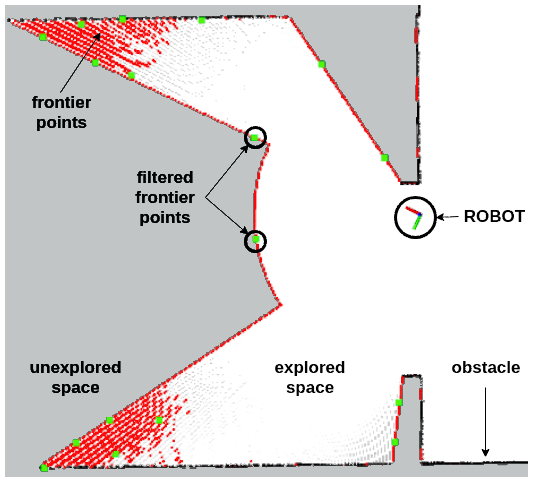
\includegraphics[width=0.85\columnwidth]{./Pictures/frontier_rviz_vol3.png}}
	\caption {The description of the environment. A 2D map is represented with an occupancy grid that divides the map into cells: the white cells describe explored and grey cells unexplored space, while the black cells define obstacles. The frontier detector publishes frontier points (red) and the filter module publishes filtered frontier points (green).}
	\label{fig:environment}
\end{figure}

\begin{figure}
    \centering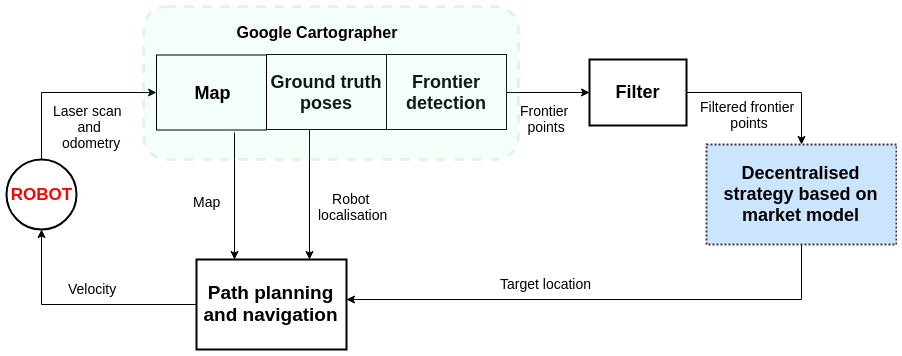
\includegraphics[width=1.0\columnwidth]{./Pictures/diagram_exploration2.png}
	\caption{Overall schematic diagram of the decentralised exploration algorithm in the simulator.}
   \label{fig:exploration-strategy}
\end{figure}

Since the main goal is to achieve faster exploration and better coordination among the mobile robots, our decentralised market-based strategy ensures that the mobile robots become dispersed throughout the environment. Moreover, the mobile robots are dispersed in the environment to accomplish the mission as fast as possible. It is assumed that communication among the mobile robots is modelled by a fully connected graph.

The rest of the paper is organised as follows. The related work is presented in the next section. In Section III the exploration strategy based on market model is described. Simulation results are presented in Section IV, and in the final section a conclusion is given.